\section{Taylor-Green vortices}

The Taylor-Green vortex sheet is a solution to the 2D Navier-Stokes
equations for an incompressible Newtonian fluid that describes a
periodic array of vortices. The vortex pattern repeats itself in the
$ x$ and$ y$ directions with a periodic length $ L$:

\begin{align*}
 u_x &= f(t) u_0 \sin k x \cos k y  \\
 u_y &= -f(t) u_0 \cos k x \sin k y ,
\end{align*}
where $ k=2\pi/L$, and the function$ f(t)$ is
\[
  f(t)= \exp(-2\nu k^2 t),
\]
so that the decay time of the vortices due to viscosity is given by
$ \tau=1/(2\nu
k^2)$. The maximum modulus of the velocity field at time zero is
$ u_0$.

The pressure field is given by
\[
  p = \frac{\rho u_0^2 }{4} f(t)^2 \left( \cos (2kx) + \cos (2ky) \right) .
\]
%
Hence the vortices go around zones of low pressure, either
clockwise or counter-clockwise (see Figure
\ref{fig:taylor-green_vortices }.)


\begin{figure}
  \centering
  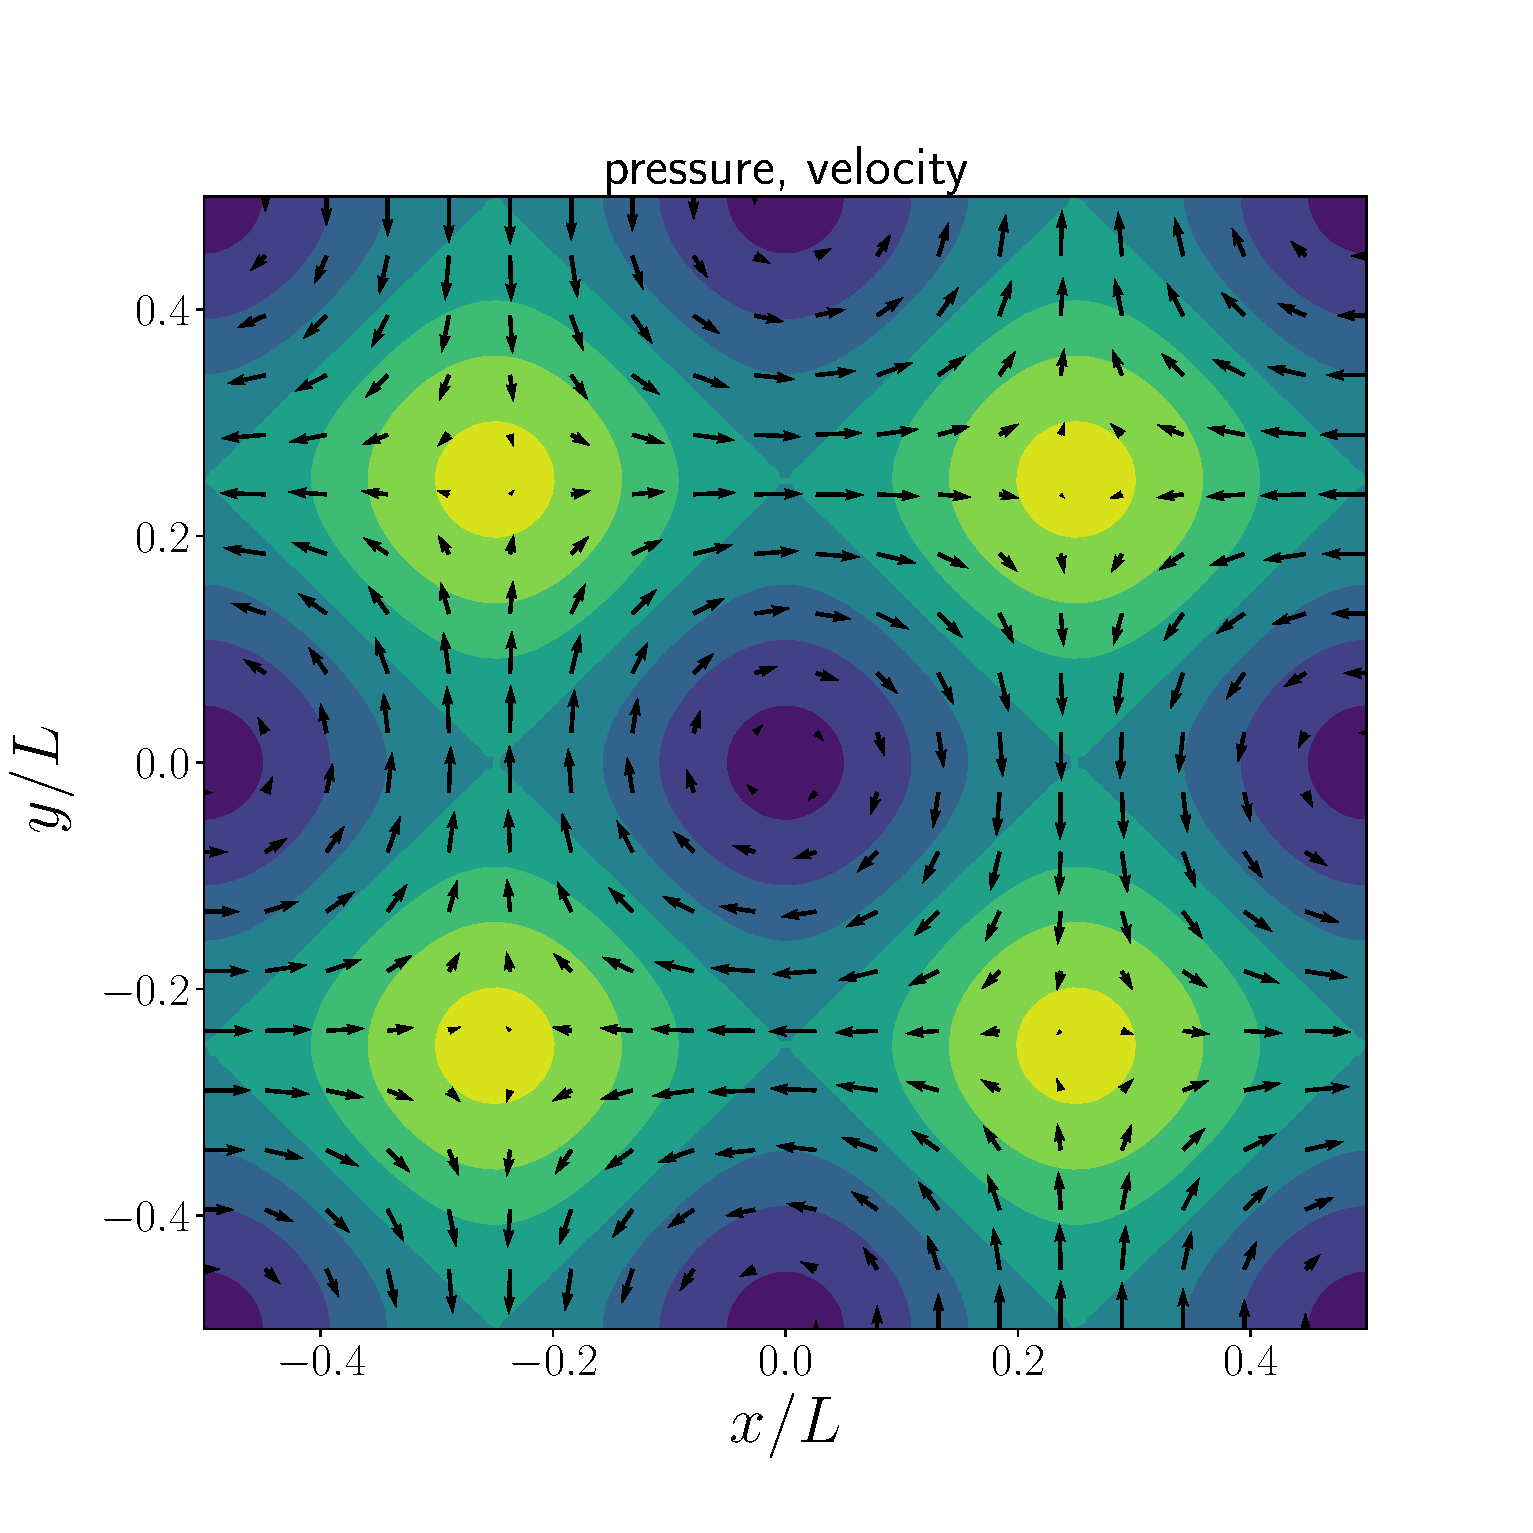
\includegraphics[width=0.4\linewidth]{figures/taylor-green_vortices}
  \caption{Taylor-Green vortices. Contour of iso-pressure (isobars),
    velocity as arrows \label{fig:taylor-green_vortices }}
\end{figure}

Insertion of these two fields into the Navier-Stokes equation shows
that indeed this is a solution. It is interesting that the pressure
gradient term exactly cancels the convective one, while the viscosity
term cancels the partial derivative. That means that in the inviscid
limit the vortices will never decay.

The vorticity field is given by
\[
  \omega = 2 f(t) \sin (kx) \sin (ky)
\]
and the stream function is just $ \psi=\omega /2$. Notice the
vorticity satisfies the convection-diffusion equation
\[
  \frac{d \omega}{d t}= \nu \nabla^2 \omega.
\]



\subsection{Reduced units}

Let us introduce the dimensionless time, built from time, maximum
initial velocity, and typical length $L$ (another choice would be
$L/2$, which is the actual length of a vortex)
\[
  t^*= t u_0 / L.
\]
Notice that $ t^*=1$ is the time a fluid particle would need to travel
a distance $L$.

Function $f$ can be written as
\[
  f(t)= \exp(-2\nu (2\pi/L)^2 (L t^* / L) ) = \exp(-8 \pi^2 t^* / \mathrm{Re}) ,
\]
%
where the Reynolds number appears naturally:
%
\[
  \mathrm{Re} := L u_0 / \nu .
\]

The decay time is then seen to be $ \tau^*=\mathrm{Re}/(8\pi^2)$ in
reduced units.


